\documentclass[a4paper, 12pt]{report}
\usepackage{lmodern}
\pagestyle{plain}
%\usepackage{textcomp}
%\usepackage{tikz}
\usepackage[table]{xcolor}
\usepackage{paralist}
%\usepackage{wrapfig}
%\newcommand*\circled[1]{\textcircled{\footnotesize#1}\normalsize}
\usepackage[T1]{fontenc}
\usepackage{polski}
\usepackage[utf8]{inputenc}
\usepackage{graphicx}
\usepackage{wrapfig}
\usepackage{sidecap}
\usepackage{titlesec}
\newcommand\cyt[1]{$^{\tiny{\cite{#1}}}$}
\newcommand\blankpage{\newpage \null \thispagestyle{empty} \addtocounter{page}{-1}}
%\usepackage[margin=4cm]{geometry}
\author{lek. Maciej Piwoda}
\title{Anestezja w chirurgii szczękowo-twarzowej}
\begin{document}
\date{}
%\maketitle
\begin{titlepage}
  \centering \vspace*{\baselineskip}
  \rule{\textwidth}{1.6pt}\vspace*{-\baselineskip}\vspace*{2pt}
  \rule{\textwidth}{0.4pt}\\[\baselineskip]
  {\LARGE Anestezja w chirurgii szczękowo-twarzowej}\\[0.2\baselineskip]
  \rule{\textwidth}{0.4pt}\vspace*{-\baselineskip}\vspace{3.2pt}
  \rule{\textwidth}{1.6pt}\\[\baselineskip]
  \scshape Praca Poglądowa do specjalizacji z anestezjologii
  i intensywnej terapii\\
  \vspace*{6\baselineskip}
  \itshape{Autor}\\
  {\large{lek. Maciej Piwoda}}\\
  \vfill
  \scshape
  Kierownik specjalizacji: lek. Maciej Gawor\\
  ordynator Oddziału Anestezjologii i Intensywnej Terapii\\
  Wojewódzkiego Centrum Medycznego w Opolu\\
  \vspace*{4\baselineskip}
  Opole 2015
\end{titlepage}
\blankpage
%\definecolor{gray75}{gray}{0.75}
\titleformat{\chapter}[block]{\LARGE\rmfamily}{\thechapter}{1em}{\titlerule\\[.5ex]\bfseries}
%\titleformat{\chapter}[hang]{\Huge\rmfamily}{\thechapter\textcolor{gray75}{|}}{0pt}{\Huge\rmfamily}
\tableofcontents
\thispagestyle{empty}
\addtocounter{page}{-1}
\blankpage
\chapter*{Wstęp}
\addcontentsline{toc}{chapter}{Wstęp}

W chirurgii szczękowo-twarzowej podobnie jak w podczas zabiegów
laryngologicznych pole działania chirurga i anestezjologa jest
wspólne, dlatego niezbędna jest między nimi ścisła współpraca.  Dostęp
do głowy pacjenta podczas operacji częstokroć nie jest możliwy. Celem
uchronienia pacjenta przed niedotlenieniem śródoperacyjnym należy
starannie zabezpieczyć układ oddechowy przed możliwością rozłączenia,
ściśle monitorować stężenia tlenu i końcowowydechowe dwutlenku węgla,
saturację krwi i obserwować pacjenta (ruchy oddechowe, kolor skóry i
krwi w polu operacyjnym). 

Pacjenci mogą być operowani z powodu wad rozwojowych, guzów twarzy,
szyi, jamy ustnej, gardła, krtani czy tchawicy, stanów zapalnych
okołoszczękowych, urazów twarzoczaszki. Mogą posiadać blizny po
urazach lub po radioterapii, które będą ograniczać ruchomość żuchwy i
podatność tkanek. Wszystkie te stany mogą w znaczącym stopniu
utrudniać intubację (jak i również wentylację przy pomocy maski
twarzowej), dlatego u tych pacjentów należy spodziewać się trudnej
intubacji.

Ekstubacja niejednokrotnie również może być wyzwaniem, ze względu na
ryzyko zachłyśnięcia krwią, ropą, czy resztkami tkanek.

\chapter{Znieczulenie w stomatologii}

Leczenie stomatologiczne odbywa się zazwyczaj bez znieczulenia lub w
znieczuleniu miejscowym. Do wykonania znieczulenia ogólnego istnieją
specjalne wskazania. Należą do nich: 
\begin{inparaenum}[\itshape a) \upshape]
\item sanacja jamy ustnej upośledzonych dzieci i dorosłych
\item jednoczasowa ekstrakcja wielu zębów
\item nacięcie ropnia okołozębowego, podżuchwowego.
\end{inparaenum}

Osoby niepełnosprawne umysłowo mogą nie współpracować i być
niespokojne, dlatego na ogół będą wymagać premedykacji przed zabiegiem
(preferowane są krótkodziałające leki sedatywne
np. midazolam). Sanację jamy ustnej najczęściej przeprowadza się w
znieczuleniu ogólnym z intubacją dotchawiczą, zazwyczaj przez nos
(lepszy dostęp do pola operacyjnego przez stomatologa), ale możliwa
jest także intubacja przez usta. Możliwe jest także zastosowanie maski
krtaniowej. Gardło uszczelnia się setonem, co pozwala na dodatkową
ochronę dróg oddechowych i zapobiega przedostawaniu się krwi i
wydzieliny do żołądka, zmniejszając w ten sposób częstość występowania
wymiotów. Oczywiście seton musi zostać usunięty przed
ekstubacją. Obecnie nie zaleca się przeprowadzania zabiegu w pozycji
siedzącej, która może powodować hipotensję. Znieczulenie regionalne
wykonane przez stomatologa pozwala ograniczyć lub całkiem zrezygnować
ze stosowania opioidów. Po zabiegu pacjent powinien pozostawać w
pozycji na boku z obniżoną głową, po to by umożliwić odpływ krwi i
śliny z jamy ustnej. W analgezji pooperacyjnej zazwyczaj się stosuje
paracetamol z niesteroidowymi lekami przeciwzapalnymi. 

\chapter{Znieczulenie do procedur w chirurgii szczękowo-twarzowej}

Jak wspomniano we wstępie podczas zabiegów chirurgii
szczękowo-twarzowej utrudniony jest dostęp do dróg oddechowych
pacjenta. Istnieje duże ryzyko zachłyśnięcia, przypadkowej ekstubacji,
zamknięcia dróg oddechowych, a w efekcie niedotlenienia
pacjenta. Dlatego wymagana jest szczególna dbałość o jak najlepsze
zabezpieczenie układu oddechowego przed rozłączeniem i bardzo
drobiazgowe monitorowanie i obserwacja pacjenta. 

Bardzo często stosuje się intubację przez nos, po ty by ułatwić
chirurgowi dostęp do pola operacyjnego. Podczas wizyty
przedoperacyjnej należy sprawdzić drożność przewodów nosowych, zapytać
o ewentualne samoistne krwawienia z nozdrzy i stosowanie leków
przeciwkrzepliwych. W przypadku prostych i krótkich zabiegów wewnątrz
jamy ustnej możliwe jest zastosowanie zbrojonej maski krtaniowej, ale
w takich przypadkach należy się liczyć z utrudnionym dostępem do pola
operacyjnego dla operatora oraz z możliwością przemieszczenia maski
krtaniowej wskutek manipulacji chirurgicznych, dlatego należy zachować
niezwykłą czujność. W przypadku jednostronnych zabiegów w obrębie jamy
ustnej jest możliwe zastosowanie intubacji przez usta i następnie
umieszczenie rurki intubacyjnej po stronie przeciwnej do pola
operacyjnego.

Należy pamiętać o zabezpieczeniu gałek ocznych, które przykryte
chustami operacyjnymi są narażone na uszkodzenia
mechaniczne. Dodatkowo zabezpieczenie dróg oddechowych przed
zanieczyszczeniem krwią, wydzieliną i resztkami tkanek można osiągnąć
stosując setony umieszczane w gardle.

Po zabiegu zawsze należy przeprowadzić laryngoskopię, by usunąć
pozostałą w gardle krew i wydzielinę oraz upewnić się, że usunięto
wszystkie setony. Esktubacja powinna być przeprowadzona u pacjenta
leżącego na boku, z głową skierowaną w dół. Niektórzy anestezjolodzy
preferują ekstubację u śpiącego, lecz już spontanicznie oddychającego
pacjenta, inni ekstubują pacjenta w pełni wybudzonego. W przypadku
intubacji przez nos rurkę intubacyjną można przekształcić w rurkę
nosowo-gardłową. Podciąga się ją tak by koniec dystalny pozostał w
gardle (ok. 15cm) i wystającą poza nos część odcina, zabezpieczając
koniec proksymalny przed możliwością wsunięcia do
nozdrza.\cyt{oxford}.

\section{Korekcja wad zgryzu}

Pacjenci operowani z powodu wad zgryzu mogą mieć jedynie nieprawidłowo
wykształconą żuchwę lub też posiadać liczne deformacje kości
twarzoczaszki, powodujące ich nieprawidłowe wzajemne
ustawienie. Częstokroć wymagają wcześniejszych ekstrakcji zębów i/lub
korekcji ortodontycznych. Zabiegi korygujące wady zgryzu mogą być
kilkuetapowe. Zazwyczaj są dość długie i trwają po kilka godzin. Mogą
się wiązać ze znaczną utratą krwi. Podczas niektórych z tych zabiegów
śródoperacyjnie pobiera się szpik kostny (zazwyczaj z talerza kości
biodrowej). Typowy pacjent do tego zabiegu to najczęściej osoba
kilkunasto- lub dwudziestoparoletnia, zazwyczaj zdrowa.

W przypadku osteotomii żuchwy często unieruchamia się ją przy pomocy
wyciągu szczękowo-żuchwowego, za pomocą specjalnych drutów. Jest to
bardzo ryzykowne, gdyż w przypadku wymiotów lub krwawienia w jamie
ustnej może dojść do zamknięcia dróg oddechowych i uduszenia się
pacjenta. Przy pacjencie zawsze powinno być specjalne narzędzie do
natychmiastowego przecięcia drutów i usunięcia wyciągu. W przypadku
gdy dojdzie do obturacji dróg oddechowych, a brakuje\footnote{co
  absolutnie nie powinno mieć miejsca} tego narzędzia należy wykonać w
trybie ratunkowym konikotomię lub konikopunkcję. U takich pacjentów
bardzo ryzykowna jest także ekstubacja, dlatego należy ją wykonać po
całkowitym powrocie stanu świadomości i siły mięśniowej u pacjenta.
Alternatywą jest stosowanie elastycznego wyciągu za pomocą specjalnych
gumek, które w nagłym przypadku łatwo i szybko da się usunąć.

Znieczulenie do tych zabiegów jest ogólne i bezwzględnie wymagana jest
intubacja dotchawicza przez nos. Wskazane jest zastosowanie
profilaktyki antybiotykowej. Przy braku przeciwwskazań można podać
sterydy (np. deksametazon w dawce 8mg) celem redukcji obrzęku tkanek.
Ze względu na długość zabiegu należy chronić pacjenta przed
hipotermią. Ważne jest również monitorowanie krwawienia. W przypadku
stosowania wyciągu szczękowo-żuchwowego należy się upewnić, że
usunięto setony, a w gardle nie ma krwi i wydzieliny. Należy
zastosować również środki przeciwwymiotne np. ondansetron,
metoclopramid lub wcześniej wspomniany deksametazon. W analgezji
pooperacyjnej pacjenci będą najczęściej wymagać paracetamolu i/lub
niesteroidowych leków przeciwzapalnych oraz niewielkich dawek
opioidów.

\section{Chirurgia onkologiczna}

\subsection{Nowotwory szczęk , żuchwy i dna jamy ustnej}

Operacje te wiążą się na ogół ze znaczną utratą krwi. Często są
rozległe z resekcją szczęk i usunięciem węzłów chłonnych (operacja
Jawdyńskiego-Crailla[!!!!!!!!!]). W operacjach nowotworu dna jamy
ustnej resekowane są mięśnie, język, ślinianki podżuchwowe i część
żuchwy. Intubacja u takiego pacjenta, ze względu na naciek
nowotworowy, powodujący zmianę warunków anatomicznych, może być trudna
i należy się do niej dobrze przygotować, uwzględniając również
konieczność wykonania pilnej tracheotomii. Czasem pacjenci mogą
wymagać wykonania planowej tracheostomii przed zabiegiem. Alternatywą
dla tracheotomii jest intubacja podbródkowo-tchawicza. Pacjenci, u
których wcześniej stosowano radioterapię w tej okolicy mają
zbliznowacone tkanki miękkie szyi i dna jamy ustnej, które znacznie
ograniczają ruchomość żuchwy i podatność jamy ustnej, co w znaczącym
stopniu utrudnia intubację.  Pacjenci ze względu na ryzyko wystąpienia
niedrożności dróg oddechowych, związanych ze zmianą warunków
anatomicznych i obrzękiem tkanek miękkich zazwyczaj wymagają
przedłużonej intubacji i parodniowego pobytu w oddziale intensywnej
terapii.

\subsection{Radykalne operacje szyi}

Wyróżnia się: 
\begin{inparaenum}[\itshape a) \upshape]
\item radykalną operację szyi, polegającą na usunięciu tkanki
limfatycznej, mięśnia mostkowo-sutkowo-obojczykowego, żyły szyjnej
wewnętrznej, nerwu dodatkowego i ewentualnie gałązek splotu szyjnego,
\item funkcjonalną radykalną operację szyi, z zachowaniem mięśnia
mostkowo-sutkowo-obojczykowego, żyły szyjnej wewnętrznej i nerwu
dodatkowego.
\end{inparaenum}

Są to na ogół wielogodzinne zabiegi, które mogą być powikłane znaczącą
utratą krwi. Nie jest błędem zastosowanie bezpośredniego monitorowania
ciśnienia tętniczego krwi, pomiaru ośrodkowego ciśnienia żylnego (po
kaniulacji żyły centralnej) i diurezy. Należy zabezpieczyć co najmniej
2 jednostki skrzyżowanej krwi. 

Należy pamiętać o możliwości ucisku na zatokę szyjną podczas
manipulacji chirurgicznych. Może to prowadzić do bradykardii i spadku
ciśnienia tętniczego, a w skrajnych przypadkach do nagłego zatrzymania
krążenia. Postępowanie polega na zaprzestaniu ucisku i podaniu
dożylnym atropiny. Profilaktycznie operator może zastosować blokadę
zatoki szyjnej za pomocą środka znieczulającego miejscowo.

Ze względu na otwarcie dużych żył szyjnych może dojść do zatoru
powietrznego.

Podczas pierwszych 48-72 godzin istnieje ryzyko pojawienia się krwiaka
lub obrzęku tkanek miękkich, które mogą doprowadzić do ucisku na drogi
oddechowe.

\section{Urazy czaszkowo-twarzowe}

Ciężkie urazy twarzoczaszki często są zagrożeniem dla drożności dróg
oddechowych, z powodu nasilonego krwawienia, wyłamanych zębów,
niestabilnych złamań, krwiaka w tkankach miękkich lub obrzęku,
szczególnie niebezpieczne jest to u pacjentów nieprzytomnych. W
przypadku złamania żuchwy może dojść do szczękościsku, który znacznie
utrudnia intubację. Złamaniom szczeki bardzo często towarzyszy
krwawienie z nosa, a u 1/4 pacjentów dochodzi do wycieku płynu
mózgowo-rdzeniowego. Przemieszczenie złamanej szczęki w kierunku
tylnej ściany gardła na ogół utrudnia w istotny sposób oddychanie
przez nos.

Pierwsza pomoc po urazie twarzoczaszki polega na udrożnieniu dróg
oddechowych, które polegać może na przytrzymaniu języka, albo szczęki,
niskim ułożeniu głowy i obróceniu jej na boku. Należy ostrożnie
odessać zawartość jamy ustnej i gardła, uważając na obluzowane zęby
delikatnie założyć rurkę ustno-gardłową. Pacjentów nieprzytomnych
należy oczywiście zaintubować. Przy urazach środkowej części twarzy
obowiązuje zakaz intubacji i zakładania sondy dożołądkowej drogą przez
nos (ze względu na ryzyko wprowadzenia rurki do mózgowia przez
szczelinę złamania). Należy wykluczyć uraz śródczaszkowy.

\subsection{Złamania żuchwy}

Operacyjna repozycja złamania żuchwy wymaga intubacji przez nos,
oczywiście po wykluczeniu złamania środkowej części twarzoczaszki. W
przypadku złamań w obrębie dwóch pięter twarzoczaszki konieczna jest
wcześniejsza tracheotomia lub intubacja podbródkowo-tchawicza. Często
po zabiegu stosuje się unieruchomienie wyciąg szczękowo-żuchwowy ze
zdrutowaniem zębów, lub założeniem specjalnych gumek. Ta druga metoda
jest bezpieczniejsza, gdyż w przypadku zagrożenia wystąpienia
niedrożności dróg oddechowych (np. w przypadku wymiotów lub
krwawienia) nie potrzebne jest specjalne narzędzie do usunięcia
wyciągu.

U pacjenta ze złamaną żuchwą często dochodzi do szczękościsku
spowodowanego przykurczem żwaczy, najczęściej jest to jedynie
przykurcz czynnościowy związany z bólem i obrzękiem. Na ogół ustępuje
on po wprowadzeniu do znieczulenia i zwiotczeniu pacjenta, ale nie
należy zawsze na to liczyć i trzeba być przygotowanym do trudności
intubacyjnych. Często mogą również wystąpić problemy z wentylacją przy
pomocy maski twarzowej, dlatego wskazane jest zastosowanie protokołu
szybkiej indukcji i intubacji.

\subsection{Złamania szczęki}

Złamania szczeki dzieli się na 3 typy się zgodnie z klasyfikacją Le
Forta.
\begin{description}
\item [Le Fort I] - poprzeczne złamanie dolnej części szczęki,
  obejmujące obie zatoki szczękowe, dno jamy nosa, podniebienie twarde
  i wyrostki zębodołowe. Odcinek podniebienny zazwyczaj jest ruchomy i
  przemieszczony do tyłu.
\item [Le Fort II] - obejmuje złamanie typu Le Fort I, które jest
  połączone z dwoma skośnymi złamaniami przebiegającymi przez dno
  oczodołów i kości nosa. Szczęka jest przemieszczona ku tyłowi. Może
  być ruchoma lub wklinowana.
\item [Le Fort III] - dochodzi do zupełnego oderwania środkowego
  segmentu twarzoczaszki od czaszki. Szczelina złamania przechodzi
  przez oczodoły i okolicę nosowo-sitową. Twarz jest w
  charakterystyczny sposób spłaszczona - ,,twarz talerzowa'', powieki
  są obrzęknięte, obecny jest krwotok z nosa, a u 25\% pacjentów
  dochodzi również do wycieku płynu mózgowo-rdzeniowego. Może wystąpić
  podwójne widzenie i zaburzenia powonienia.
\end{description}


[Tu pierdolnę obrazek - klasyfikacja Le Forta]\newline

Tak jak i w przypadku urazów żuchwy i tu może dojść i często dochodzi
do niedrożności górnych dróg oddechowych. Pacjentów nieprzytomnych
należy zaintubować. Przeciwwskazana jest intubacja przez nos w
przypadku złamań środkowego piętra twarzoczaszki, tak samo jak i
zakładanie przez nos sondy żołądkowej, ze względu na ryzyko
umiejscowienia rurki lub sondy w zatoce szczękowej, oczodole, lub
nawet wewnątrzczaszkowo. Dopiero po odpowiedniej inspekcji nozdrzy
przy pomocy fiberoskopu można zaintubować pacjenta drogą przeznosową.
Sam zabieg polega na mobilizacji i repozycji załamanych kości, z
wewnętrzną lub zewnętrzną stabilizacją i unieruchomieniem
międzyszczękowym przy pomocy drutów lub odpowiednich gumek. Należy się
liczyć z trudnościami oddechowymi po zabiegu, szczególnie w przypadku
obrzęku przewodów nosowych - w takich przypadkach można przed
stabilizacją wprowadzić rurkę nosowo-gardłową. Należy ekstubować tylko
i wyłącznie pacjentów przytomnych, co do których mamy pewność, że mają
drożne drogi oddechowe.

\subsection{Złamania łuku jarzmowego}

Złamanie łuku jarzmowego może być złamaniem izolowanym lub
współistnieć z innymi złamaniami kości twarzoczaszki. Czasami dochodzi
do ograniczenia ruchomości w stawie skroniowo-żuchwowym, ze względu na
blokowanie wyrostka dziobiastego żuchwy przez przemieszczoną kość
jarzmową. Złamanie może być stabilne i wtedy wymaga tylko repozycji
przezskórnej przez policzek, lub niestabilne i wtedy konieczna jest
stabilizacja wewnętrzna. Dostęp może być zewnętrzny przez wspomniany
już policzek lub też z dostępu przezskroniowego, rzadziej wewnętrzny:
od strony jamy ustnej lub przedsionka nosa.  Zabieg odbywa się w
znieczuleniu ogólnym z intubacją przez usta.

\subsection{Złamania oczodołu[?]}


\section{Wrośnięty ząb[?] i ropień okołozębowy}

Zabieg na ogół jest krótki i nie wiąże się ze zbyt dużym nasileniem
dolegliwości bólowych. Ze względu na lepszy dostęp do pola
operacyjnego preferowana jest intubacja przez nos, ale możliwe jest
zastosowanie intubacji przez usta, zwłaszcza w przypadkach, gdy zabieg
dotyczy tylko jednej strony jamy ustnej (rurka intubacyjna
umiejscowiona jest wtedy po przeciwnej stronie ust). W przypadku
prostej, jednostronnej ekstrakcji można użyć maski krtaniowej.

W przypadku ropnia okołozębowego lub podżuchwowego może dojść do
szczękościsku, który może utrudniać lub nawet uniemożliwiać
przeprowadzenie intubacji. Chorzy z ropniem mogą być odwodnieni,
wyczerpani, z wysoką gorączką. Antybiotykoterapia powinna być
rozpoczęta przed zabiegiem.

Celem analgezji podczas zabiegu jak i pooperacyjnej można zastosować
blokadę odpowiednich odgałęzień nerwu trójdzielnego (odgałęzienia
nerwu szczękowego lub żuchwowego).

\chapter{Intubacja tchawiczo-podbródkowa}

Intubacja tchawiczo-podbródkowa jest alternatywną dla tracheotomii
metodą zapewnienia drożności dróg oddechowych podczas znieczulenia
ogólnego w trakcie zabiegów w zakresie środkowego i dolnego piętra
twarzy. Podczas tych operacji istnieje konieczność kontroli zwarcia
zębów i symetrii kości twarzy, co wyklucza możliwość zastosowania
intubacji bardziej tradycyjnymi drogami, tj. drogą przez nos lub usta.

Procedura intubacji tchawiczo-podbródkowej została opisano po raz
pierwszy przez Hernandeza Altemira w 1986 r\cyt{altemir}. %{W
%Wojewódzkim Centrum Medycznym w Opolu stosowana jest metoda intubacji
%tchawiczo-podbródkowej w modyfikacji profesora
%Bartkowskiego\cyt{bartkowski}\cyt{gawor}, która polega na
%wyprowadzeniu rurki w linii środkowej, a nie w okolicy podżuchwowej,
%jak proponował H. Altemir.}

Wskazania do tej procedury to:
\begin{inparaenum}[\itshape a) \upshape]
\item rozległe obrażenia górnego, środkowego i dolnego piętra twarzy
\item jednoczasowa korekcja nosa, warg oraz zmarszczek twarzy i szyi 
\item jednoczasowa osteotomia szczęk i żuchwy
\item w niektórych zabiegach onkologicznych. 
\end{inparaenum}
Przeciwwskazania natomiast to nacieki zapalne i zmiany rozrostowe dna
jamy ustnej oraz zesztywnienie stawów skroniowo-żuchwowych. Nie
stosuje się tej metody również u pacjentów nieprzytomnych lub
niewspółpracujących.

Zalety intubacji tchawiczo-podbródkowej są liczne. Jest to metoda
stosunkowo prosta i bezpieczna, umożliwia swobodny dostęp do rurki
intubacyjnej podczas trwania zabiegu, umożliwia przedłużoną intubację
w sytuacji zagrożenia pooperacyjną niedrożnością górnych dróg
oddechowych lub konieczności wspomagania wentylacji. Metoda ta jest
ceniona w chirurgii estetycznej, umożliwiając jednoczesne wykonanie
skomplikowanych procedur, takich jak korekcja zmarszczek twarzy,
rynoplastyka, modelacja warg i podbródka. Natomiast w chirurgii
szczękowo twarzowej umożliwia w trakcie trwania operacji stałą ocenę i
korektę warunków zwarciowo-zgryzowych oraz symetrii twarzy u pacjentów
po ciężkich urazach kości twarzoczaszki i z wadami gnatycznymi, którzy
wymagają jednoczesnej osteotomii korekcyjnej żuchwy i szczęk.

Oczywiście alternatywnie można wykonać tracheotomię, która jednak jest
zabiegiem dużo bardziej okaleczającym, ze znacznie liczniejszymi i
bardziej poważnymi powikłaniami, do których należą:
\begin{inparaenum}[\itshape a) \upshape]
\item krwotok z uszkodzonych naczyń
\item odma podskórna i śródpiersiowa
\item zakażenie
\item porażenie nerwów krtaniowych wstecznych
\item zwężenie krtani i/lub tchawicy
\item przetoka tchawiczo-przełykowa
\item przetoka tchawiczo-skórna
\item rozległe procesy wytwórcze z tworzeniem ziarniny.
\end{inparaenum}

Natomiast najbardziej istotne powikłania intubacji
tchawiczo-podbródkowej to:
\begin{inparaenum}[\itshape a) \upshape]
\item uszkodzenie ślinianki podjęzykowej
\item krwawienie
\item ryzyko niedotlenienia pacjenta w efekcie przypadkowej ekstubacji
  podczas zabiegu.
\end{inparaenum}


\section*{Opis procedury\footnote{Wszystkie zdjęcia tu użyte są
  autorstwa doktora Macieja Gawora i zostały tu zamieszczone za jego zgodą}}

\begin{wrapfigure}{r}{0.5\textwidth}
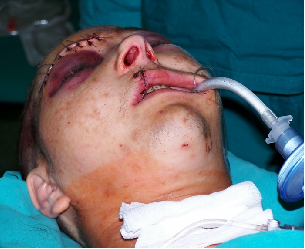
\includegraphics[width=0.4\textwidth]{images/itp1}
\end{wrapfigure}
\hfill\\
Pierwszym krokiem jest po indukcji znieczulenia intubacja pacjenta
metodą przez usta przy użyciu laryngoskopu lub fiberoskopu. Rurkę
należy przemieścić do lewego kącika ust.
\hfill\\
\hfill\\
\hfill\\
\hfill\\

\begin{wrapfigure}{r}{0.5\textwidth}
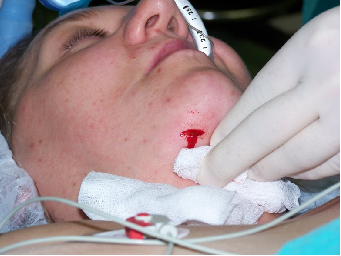
\includegraphics[width=0.4\textwidth]{images/itp2}
\end{wrapfigure}

\hfill\\
Następnie po przygotowaniu i umyciu pola zabiegu znieczula się przy
użyciu środka miejscowo znieczulającego skórę okolicy podbródkowej, w
linii środkowej, doogonowo od naturalnego fałdu skóry.  W tym miejscu
należy wykonać 1,5 centymetrowe nacięcie.

\newpage
\hfill\\
\hfill\\
\hfill\\

\begin{wrapfigure}{r}{0.5\textwidth}
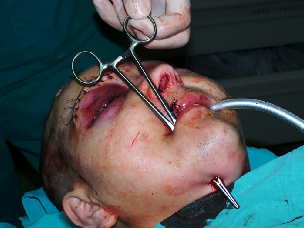
\includegraphics[width=0.4\textwidth]{images/itp3}
\end{wrapfigure}

\hfill\\
Kolejnym etapem jest rozwarstwienie tkanek dna jamy ustnej przy użyciu
kleszczy Peana. Kleszcze przekłada się od strony jamy ustnej, tak by
by ich końce wystawały przez skórę z wytworzonego otworu. Otwór w
dnie jamy ustnej powinien znajdować się na wysokości dolnych siekaczy,
bocznie od wędzidełka języka i do przodu od ujść przewodów Whartona.
\hfill\\

\begin{wrapfigure}{r}{0.5\textwidth}
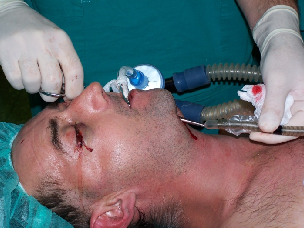
\includegraphics[width=0.4\textwidth]{images/itp3a}
\end{wrapfigure}

\hfill\\
Następnie należy przeciągnąć przez powstały otwór drugą rurkę
intubacyjną (rurka zbrojona) za jej koniec dystalny.
\hfill\\
\hfill\\
\hfill\\
\hfill\\
\hfill\\
\hfill\\

\begin{wrapfigure}{r}{0.5\textwidth}
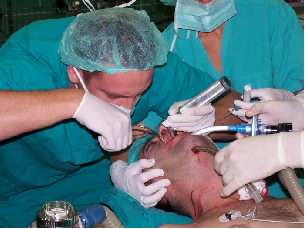
\includegraphics[width=0.4\textwidth]{images/itp4}
\end{wrapfigure}

\hfill\\
Po wprowadzeniu rurki do gardła. Usuwa się z krtani pierwszą rurkę i
następnie intubuje się pacjenta rurką drugą.

\newpage
\hfill\\
\hfill\\
\hfill\\
\hfill\\
\hfill\\

\begin{wrapfigure}{r}{0.5\textwidth}
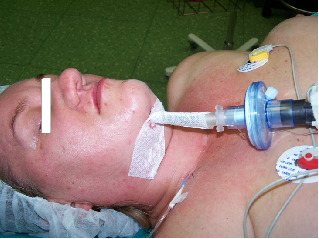
\includegraphics[width=0.4\textwidth]{images/itp5}
\end{wrapfigure}

\hfill\\
Po ustaleniu właściwej głębokości rurka jest fiksowana do skóry przy
pomocy plastrów. Można również użyć szwu nylonowego o grubości 3.0.

\hfill\\
\hfill\\
\hfill\\
\hfill\\
\hfill\\

Alternatywnie można użyć tylko jednej rurki (bez etapu
przeintubowania pacjenta). Przeciąga się wtedy koniec proksymalny
(najpierw kontrolny balonik z przewodem do uszczelnienia mankietu)
przez wytworzony kanał. W takim przypadku najpierw należy usunąć
łącznik z końca proksymalnego rurki.

Po ekstubacji ranę skóry zaopatruje się szwem grubości 5.0, a ranę
błony śluzowej dna jamy ustnej szwem 4.0 lub też zostawia się ją bez
zaopatrzenia. Jeśli rodzaj zabiegu lub stan pacjenta tego wymaga można
bezpiecznie rurkę pozostawić na okres do 72 godzin.\cyt{bartkowski}

\begin{thebibliography}{99}
\addcontentsline{toc}{chapter}{Bibliografia}
\bibitem{oxford} oxford
\bibitem{larsen} larsen
\bibitem{zawadzka} zawadzka
\bibitem{altemir} Hernandez Altemir F.: The submental route for
  endotracheal intubation. A new technique. Journal of Oral and
  Maxillo-Facial Surgery [!!!!!!!!!!!!!!!!]
\bibitem{bartkowski} Bartkowski S., Bartkowski J. i wsp.:Polski
  Przegląd Chirurgiczny; czerwiec 2001, t73, 521-528
\bibitem{gawor} gawor
\end{thebibliography}
\end{document}